\documentclass{standalone}
\usepackage[dvipsnames]{xcolor}
\usepackage{tikz}                       % Graphen und kommutative Diagramme
\usetikzlibrary{patterns}               % Um schraffierte Formen in der tikzpicture-Umgebung zu zeichnen.
\newcommand{\ul}[1]{\underline{\smash{#1}}}

\begin{document}
\centering
\begin{minipage}{.4\textwidth}
\centering
\resizebox{!}{4.5cm}{
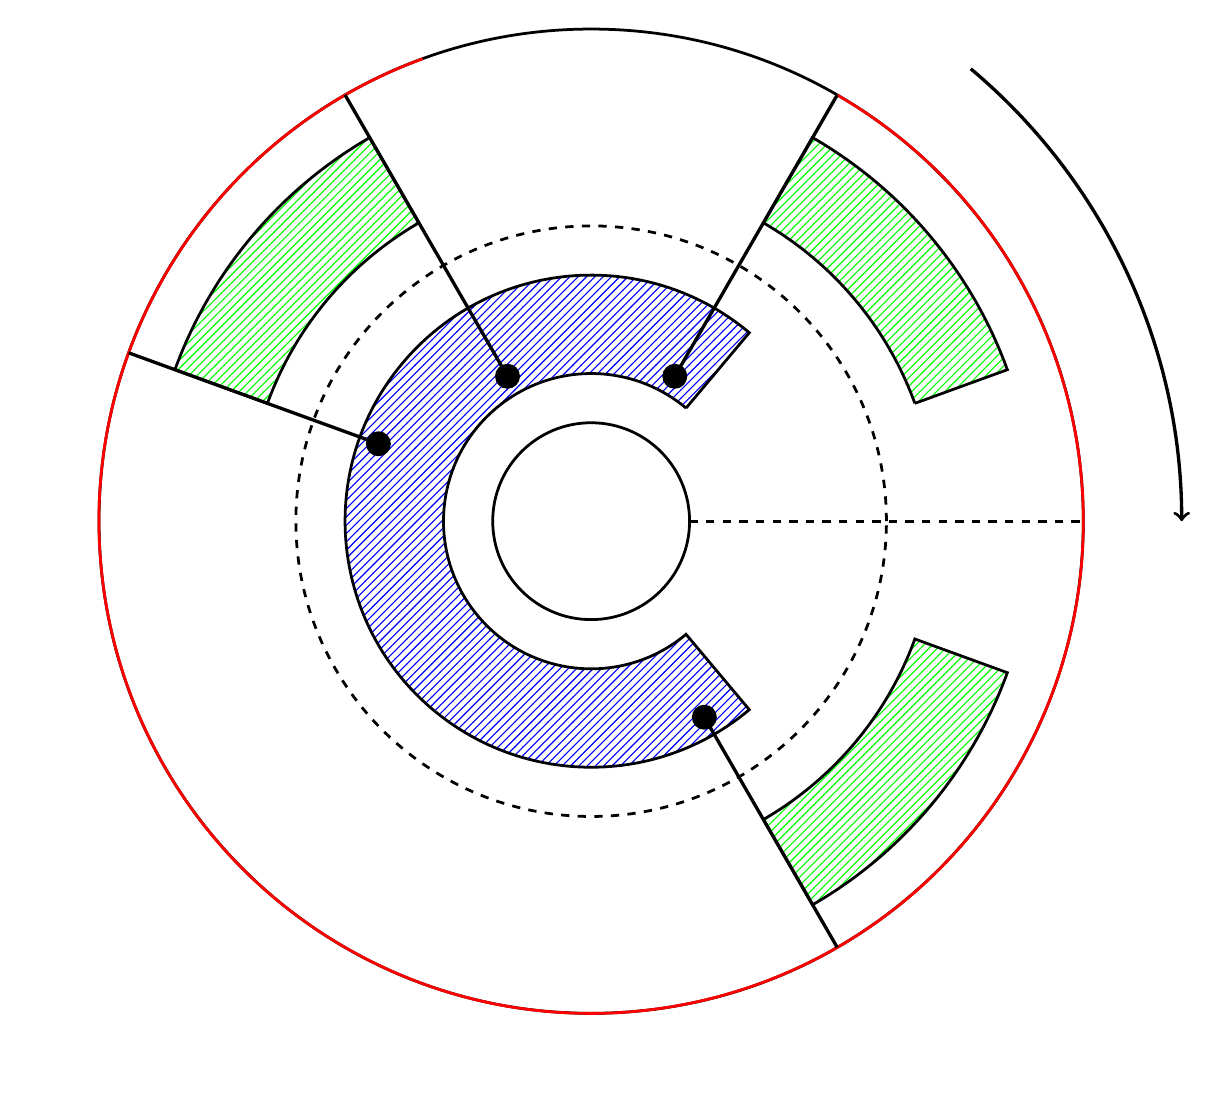
\begin{tikzpicture}[x=1.25cm, y=1.25cm, line width=1pt]
    % draw inner and outer circles
    \draw[color=black] (0, 0) circle (1);
    \draw[color=black] (0, 0) circle (5);
    \draw[color=black, dashed] (0, 0) circle (3);
    \draw[color=red] (60 : 5) arc [radius = 5, start angle = 60, delta angle = -310];

    % draw 0 line
    \draw[color=black, dashed] (0 : 1) -- (0 : 5); 
    
    % draw shaded slit box
    \filldraw[pattern=north east lines, pattern color=blue] 
      (50 : 1.5) -- (50 : 2.5) arc [radius = 2.5, start angle = 50, delta angle = 260] 
	       -- (310 : 1.5) arc [radius = 1.5, start angle = 310, delta angle = -260] ; 
    
    \filldraw[pattern=north east lines, pattern color=green] 
      (300 : 3.5) -- (300 : 4.5) arc [radius = 4.5, start angle = 300, delta angle = 40] 
	       -- (340 : 3.5) arc [radius = 3.5, start angle = 340, delta angle = -40];
    \filldraw[pattern=north east lines, pattern color=green] 
      (20 : 3.5) -- (20 : 4.5) arc [radius = 4.5, start angle = 20, delta angle = 40] 
	       -- (60 : 3.5) arc [radius = 3.5, start angle = 60, delta angle = -40];
    \filldraw[pattern=north east lines, pattern color=green] 
      (120 : 3.5) -- (120 : 4.5) arc [radius = 4.5, start angle = 120, delta angle = 40] 
	       -- (160 : 3.5) arc [radius = 3.5, start angle = 160, delta angle = -40];
	       
     % draw slits
    \draw[color=black, line width=1.2pt] (60 : 5) -- (60 : 1.7);
    \filldraw[color = black, fill = black] (60 : 1.7) circle (4pt);

    \draw[color=black, line width=1.2pt] (160 : 5) -- (160 : 2.3);
    \filldraw[color = black, fill = black] (160 : 2.3) circle (4pt);
     
    \draw[color=black, line width=1.2pt] (300 : 5) -- (300 : 2.3);

    \filldraw[color = black, fill = black] (300 : 2.3) circle (4pt);
     
    \draw[color=black, line width=1.2pt] (120 : 5) -- (120 : 1.7);
    \filldraw[color = black, fill = black] (120 : 1.7) circle (4pt);
    
    \draw[->, line width=1.2pt] (50 : 6) arc[radius = 6, start angle = 50, delta angle = -50];
    \end{tikzpicture}
}
\end{minipage}
\centering

\begin{minipage}{.4\textwidth}
\centering
\resizebox{!}{4.5cm}{
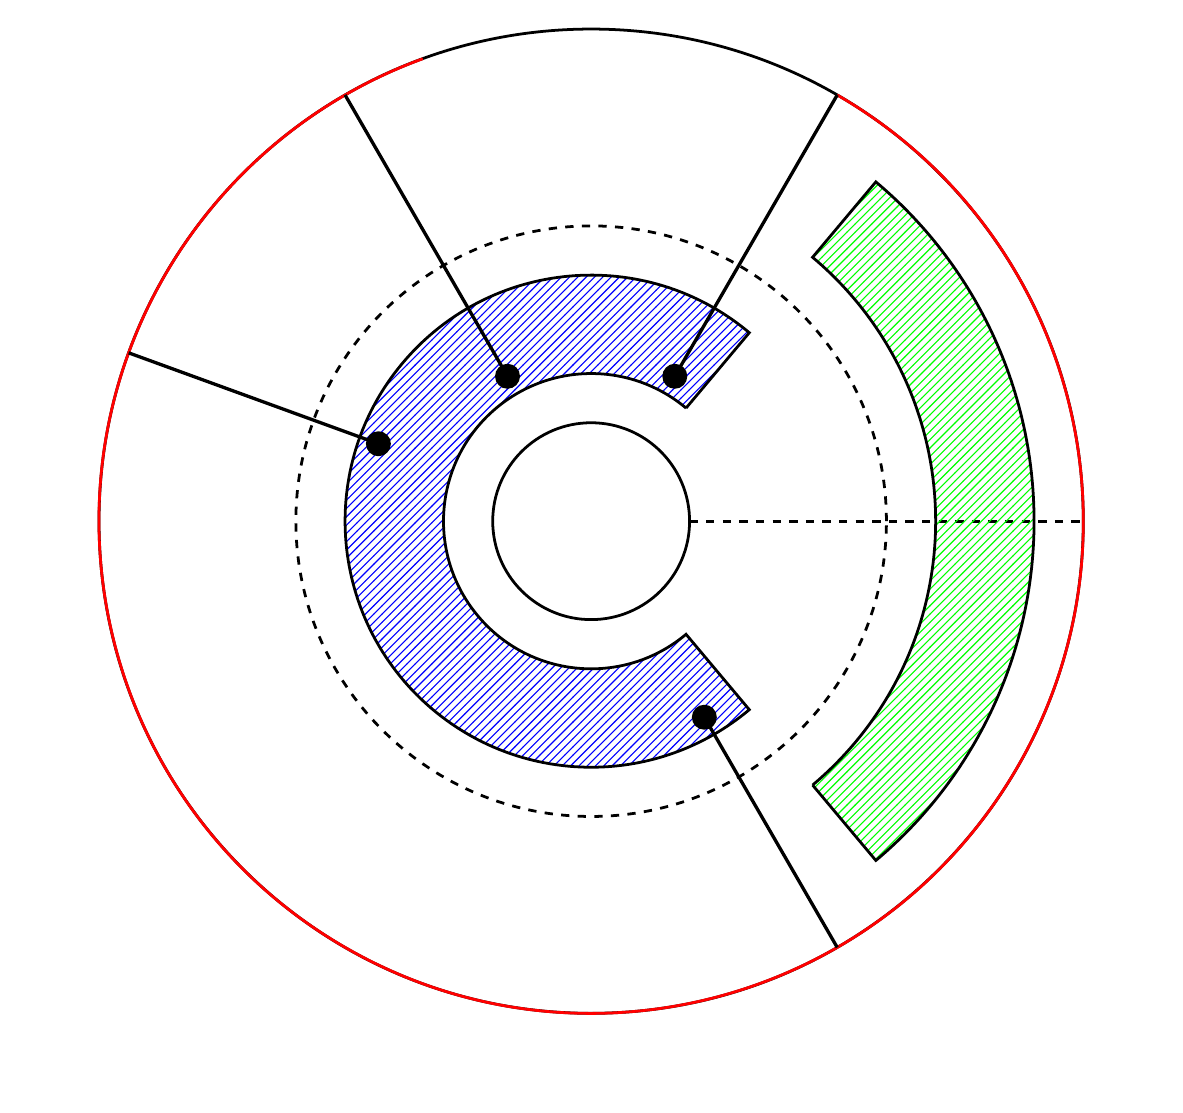
\begin{tikzpicture}[x=1.25cm, y=1.25cm, line width=1pt]
    % draw inner and outer circles
    \draw[color=black] (0, 0) circle (1);
    \draw[color=black] (0, 0) circle (5);
    \draw[color=black, dashed] (0, 0) circle (3);
    \draw[color=red] (60 : 5) arc [radius = 5, start angle = 60, delta angle = -310];

    % draw 0 line
    \draw[color=black, dashed] (0 : 1) -- (0 : 5); 
    
    % draw shaded slit box
    \filldraw[pattern=north east lines, pattern color=blue] 
      (50 : 1.5) -- (50 : 2.5) arc [radius = 2.5, start angle = 50, delta angle = 260] 
	       -- (310 : 1.5) arc [radius = 1.5, start angle = 310, delta angle = -260] ; 
    
    \filldraw[pattern=north east lines, pattern color=green] 
      (310 : 3.5) -- (310 : 4.5) arc [radius = 4.5, start angle = 310, delta angle = 100] 
	       -- (50 : 3.5) arc [radius = 3.5, start angle = 50, delta angle = -100];

	       % draw slits
    \draw[color=black, line width=1.2pt] (60 : 5) -- (60 : 1.7);
    \filldraw[color = black, fill = black] (60 : 1.7) circle (4pt);

    \draw[color=black, line width=1.2pt] (160 : 5) -- (160 : 2.3);
    \filldraw[color = black, fill = black] (160 : 2.3) circle (4pt);
     
    \draw[color=black, line width=1.2pt] (300 : 5) -- (300 : 2.3);

    \filldraw[color = black, fill = black] (300 : 2.3) circle (4pt);
     
    \draw[color=black, line width=1.2pt] (120 : 5) -- (120 : 1.7);
    \filldraw[color = black, fill = black] (120 : 1.7) circle (4pt);
 
\end{tikzpicture}
}
\end{minipage}


\end{document}
